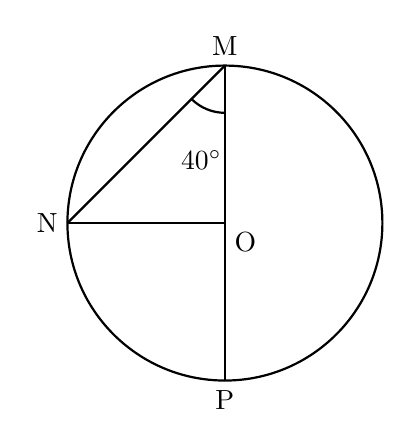
\begin{tikzpicture}[scale=1]

    % Define the radius of the circle
    \def\R{2}

    % Define the center of the circle
    \coordinate (O) at (0,0);

    % Draw the circle
    \draw[thick] (O) circle (\R);

    % Define points on the circle
    % P is at the bottom (-90 degrees)
    \coordinate (P) at (0,-\R);
    % M is at the top (90 degrees)
    \coordinate (M) at (0,\R);
    % N is on the left side, exactly horizontally aligned with O
    \coordinate (N) at (-\R,0);

    % Draw the lines
    \draw[thick] (M) -- (P); % Diameter MP
    \draw[thick] (N) -- (O); % Radius NO
    \draw[thick] (N) -- (M); % Chord NM

    % Draw the angle arc at M
    % Start angle is from M to N, end angle is from M to O (which is straight down, -90 degrees)
    % Angle from M(0,2) to N(-2,0) is 225 degrees.
    % We want the arc between the line MN and the line MO.
    \draw[thick] (M) ++(-90:0.6) arc (-90:-135:0.6);

    % Add the angle label
    \node at (-0.3, 0.8) {$40^\circ$};

    % Label the points
    \node[above] at (M) {M};
    \node[left] at (N) {N};
    \node[below] at (P) {P};
    \node[below right] at (O) {O};

\end{tikzpicture}